%%%%%%%%%%%%%%%%%%%%%%%%%%%%%%%%%%%%%%%%%%%%%%%%%%%%%%%%%%%%%%%%%%%%%%%%%%%%%%%%
%2345678901234567890123456789012345678901234567890123456789012345678901234567890
%        1         2         3         4         5         6         7         8

\documentclass[letterpaper, 10 pt, conference]{ieeeconf}  % Comment this line out
                                                          % if you need a4paper
%\documentclass[a4paper, 10pt, conference]{ieeeconf}      % Use this line for a4
                                                          % paper

\IEEEoverridecommandlockouts                              % This command is only
                                                          % needed if you want to
                                                          % use the \thanks command
\overrideIEEEmargins
% See the \addtolength command later in the file to balance the column lengths
% on the last page of the document



% The following packages can be found on http:\\www.ctan.org
%\usepackage{graphics} % for pdf, bitmapped graphics files
%\usepackage{epsfig} % for postscript graphics files
%\usepackage{mathptmx} % assumes new font selection scheme installed
%\usepackage{times} % assumes new font selection scheme installed
\usepackage{amsmath} % assumes amsmath package installed
\usepackage{amssymb}  % assumes amsmath package installed
\usepackage{boldline}
\usepackage{array,multirow}
\usepackage{dblfloatfix} 
\usepackage{hyperref}
\usepackage{float}
\usepackage{color}
\usepackage{xfrac}
\usepackage{graphicx}
\graphicspath{ {images/} }
\definecolor{light-gray}{gray}{0.95}
\newcommand{\code}[1]{\colorbox{light-gray}{\texttt{#1}}}
\DeclareMathOperator*{\argmax}{arg\,max}
\DeclareMathOperator*{\maxU}{max}
\usepackage{makecell}
\usepackage{bbm}
\usepackage[table,xcdraw]{xcolor}
\usepackage[flushleft]{threeparttable}
\usepackage[utf8]{inputenc}
\usepackage{capt-of}
\usepackage{mathrsfs}


\title{\LARGE \bf
A Closer Look At The Convergence of Adam and AMSGrad:\\A Reproduction Study
}

\author{ 
	\parbox{2 in}{\centering Tamir Bennatan
         {\tt\small tamir.bennatan@mail.mcgill.ca\\}
         {\tt\small 260614526}}
         \hspace*{ 0.3 in}
         \parbox{2 in}{\centering Lea Collin
         {\tt\small lea.collin@mail.mcgill.ca\\}
         {\tt\small 260618407}}
         \hspace*{0.3 in}
         \parbox{2 in}{\centering Emmanuel Ng Cheng Hin
         {\tt\small emmanuel.ngchenghin@mail.mcgill.ca\\}
         {\tt\small 260615964}}
}



\begin{document}



\maketitle
\thispagestyle{empty}
\pagestyle{empty}

%%%%%%%%%%%%%%%%%%%%%%%%%%%%%%%%%%%%%%%%%%%%%%%%%%%%%%%%%%%%%%%%%%%%%%%%%%%%%%%%


%%%%%%%%%%%%%%%%%%%%%%%%%%%%%%%%%%%%%%%%%%%%%%%%%%%%%%%%%%%%%%%%%%%%%%%%%%%%%%%%
\section{INTRODUCTION}

	The authors of the paper present issues with the popular stochastic gradient descent optimizers: RMSProp and ADAM, focusing mainly on ADAM. ADAM uses exponential moving averages of squared past gradients, which limits the reliance of parameter updates to only the last few gradients. Though ADAM has been proven to be very useful in many settings, it has also been shown to fail to converge to optimal solutions in certain cases. The usual problem in these other cases is that large, informative gradients during updates occur infrequently. Because ADAM limits the reliance of parameter updates to only the past few gradients, the influence of these informative gradients quickly die out due to the use of exponential moving averages, leading to poor convergence. \par
    The paper introduces a toy example where it is obvious that ADAM does not converge to the optimal solution. The authors go on to discuss an incorrect assumption in the proof of convergence of ADAM that illuminates why ADAM does not converge in certain cases. Finally, the authors present a solution to the issue: AMSGrad. Their solution takes into consideration the ``long-term'' past history of gradients, so as not to lose the informative yet rare gradients that occur. The authors ran several experiments and compared the performance on training and test loss of both ADAM and AMSGrad. In this reproduction study, we aim to recreate these results as best as possible, while taking into consideration the cost of doing so. Additionally, we seek to identify any shortcomings or oversights of the authors. 
     
\section{THE NON-CONVERGENCE OF ADAM}
The authors of this paper discuss in detail the issue with ADAM and point out an error in ADAM's proof of convergence. The quantity of interest in the proof is:
$$
	\Gamma_{t+1} = \Bigg(\frac{\sqrt{V_{t+1}}}{\alpha_{t+1}} - \frac{\sqrt{V_{t}}}{\alpha_{t}} \Bigg) 
$$

This quantity essentially measures the change in the inverse of the learning rate of the adaptive method with respect to time. The update rules of stochastic gradient descent lead to ``non-increasing'' learning rates. What the authors point out, however, is that ADAM and RMSProp can have potentially indefinite $\Gamma_{t}$, which leads to a lack of convergence. The authors claim that this problem arises because algorithms like ADAM use exponential moving averages. \par
The authors present a toy, adversarial example to illustrate their point on why ADAM fails to converge. The example is as follows, for $\mathcal{F} = [-1, 1]$:
\[
    f_{t}(x) = 
    \begin{cases}
     	Cx, \hspace{5mm} \text{for } t \text{ mod 3 = 1} \\
        -x, \hspace{5mm} \text{otherwise}
    \end{cases}
\]
where $C>2$. It is easy to see that the value of $x$ that leads to the minimum regret is $-1$, however, the authors show that ADAM converges to the highly suboptimal solution of $x = +1$. This elucidates the intuition that the influence of the large gradient $C$ disappears too quickly to counteract the gradient of $-1$, which moves the algorithm in the wrong direction. \par
As a solution to ADAM's shortcomings, the authors use a smaller learning rate in comparison to ADAM that still incorporates the intuition of slowly decaying the effect of past gradients on the learning rate, as long as $\Gamma_{t}$ is positive semidefinite. The solution they present is AMSGrad. 

\section{METHODOLOGY}
The authors ran several experiments to compare the performance of ADAM and AMSGrad. We wanted to recreate every experiment the authors ran, as closely as possible, in order to assess the reproducibility and validity of their results. 
\par The first two experiments they did, which they refer to as synthetic experiments, are very similar to the toy example they used to show the non-convergence of ADAM. The first synthetic experiment is with an online setting:

\[
    f_{t}(x) = 
    \begin{cases}
     	1010x, \hspace{5mm} \text{for } t \text{ mod 101 = 1} \\
        -10x, \hspace{5mm} \text{otherwise}
    \end{cases}
\]

while the second is with a stochastic setting:

\[
    f_{t}(x) = 
    \begin{cases}
     	1010x, \hspace{5mm} \text{with probability 0.01}\\
        -10x, \hspace{5mm} \text{otherwise}
    \end{cases}
\]

with both having the constraint set $\mathcal{F} = [-1, 1]$. Very similar to the general toy example, the optimal solutions are both clearly $x = -1$ and so the algorithms are expected to converge to this optimal value. \par
For these experiments, we aimed to recreate this experiment with both settings with the goal of reproducing the figures the authors included. The authors' results are shown in Figure 1. 

\begin{figure*}[]
\centering
\begin{minipage}{0.9\textwidth}
  \centering
  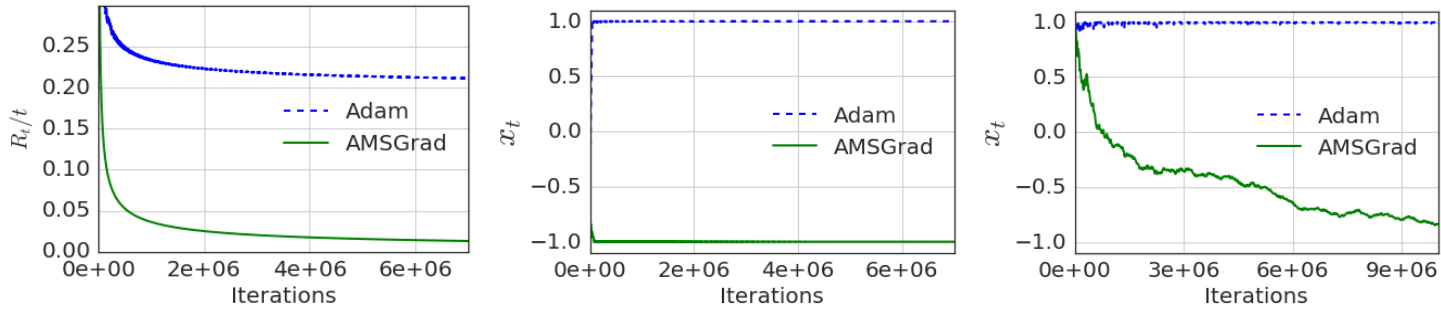
\includegraphics[width=1\linewidth]{OG_Results_synth.png}
  \label{fig:test1}
\end{minipage}%
\caption[]{The left two plots (left and center) are for the online setting and the last one (right) is for the stochastic setting. Note: these graphs were taken directly from the paper.}
\end{figure*}

To implement these synthetic experiments, we used the same values for $\beta_{1}$ and $\beta_{2}$ as the authors, 0.9 and 0.99, respectively, for both ADAM and AMSGrad. As the authors did, we looked at the regret and the value of the iterate $x_{t}$ for both algorithms. To find a ``good'' value for $\alpha$ we did a by-hand search through several values. (NEED TO ELABORATE ON THIS - ASK EMMANUEL). \par
The authors then investigated the performance of the algorithm on a logistic regression problem. They used the MNIST dataset, which contains 784 dimensional image vectors that each belong to one of 10 classes. The authors are clear in describing the step size parameter they chose ($\alpha / \sqrt{t}$), the minibatch size (128), and $\beta_{1}$ (0.9). They do not specify the values of $\beta_{2}$ and $\alpha$ that they tried, however, they do mention that they chose these values using a grid search and they give the range of values they tried for $\beta_{2}$ (0.99 - 0.999). We initially ran one experiment of logistic regression with set values for all of the hyperparameters to confirm that these algorithms behave similarly to the way that the authors described, before we started looking at many different values. \par
The authors then looked at the performance of ADAM and AMSGrad on different neural networks. They trained a 1-hidden layer, fully connected neural network on MNIST. Once again they specify that they used $\beta_{1} = 0.9$ and the range of $\beta_{2}$ that they tried (0.99 - 0.999). They also specify that they used 100 ReLU nodes in the hidden layer for the experiment and that they used a constant $\alpha_{t} = \alpha$. They again say that they performed a grid search to look through ranges of $\alpha$ and $\beta_{2}$. \par
As a final experiment, the authors trained a convolutional neural network (CNN) on the standard CIFAR-10 dataset, which consists of 60,000 labeled 32 by 32 images. They specify the architecture that they used which has 2 convolutional layers with 64 channels and a kernel size of 6 by 6 followed by 2 fully connected layers of size 384 and 192. The network uses a 2 by 2 max pooling and layer response normalization between the convolutional layers. A dropout layer with keep probability of 0.5 was applied in between the fully connected layers. Once again, the minibatch size was set to 128, the same as the previous experiments. We followed the architecture almost exactly, though we used batch normalization rather than the layer response normalization the authors used. Again, they state that they used a grid search to iterate through different values of $\alpha$ and $\beta_{2}$. The results from the paper can be seen in Figure 2. \par
Overall, we tried to replicate as much as possible what the authors did. Once we had found the best hyperparameters (namely, $\alpha$ and $\beta_{2}$) as a result of our grid search, we ran each algorithm 5 times and plotted the training and test losses for each ``run''. We thought this was important to do as each algorithm has random initializations and can randomly get ``stuck'' sometimes while running. Performing each experiment allows us to see if perhaps the authors hand-picked results that went along with their hypothesis or if the results really were consistent, even after taking into consideration the randomness of the algorithms. 
    
\begin{figure*}[]
\centering
\begin{minipage}{0.9\textwidth}
  \centering
  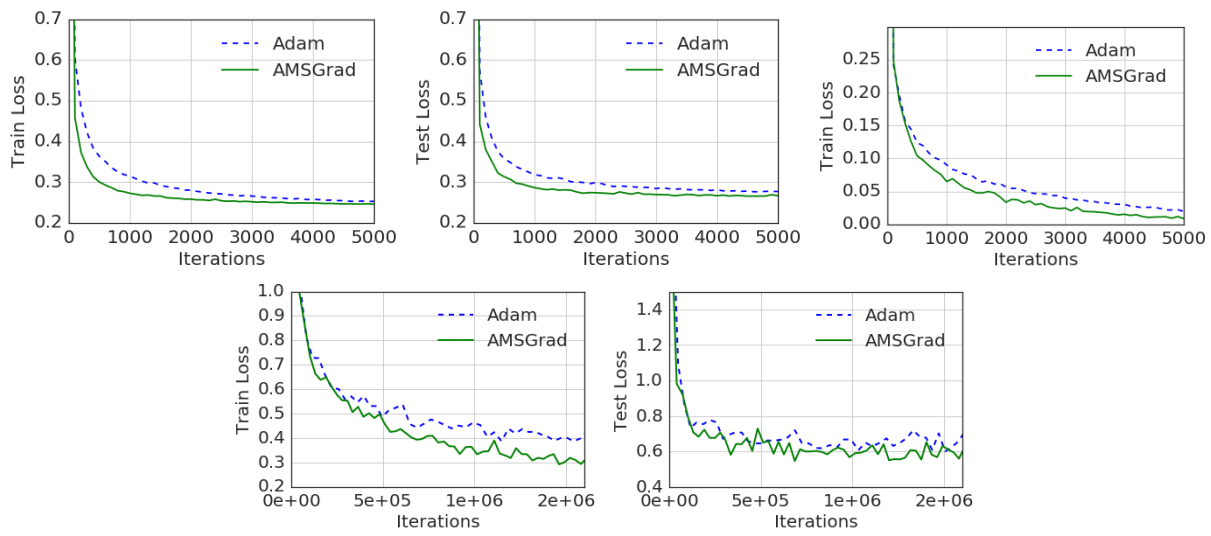
\includegraphics[width=1\linewidth]{OG_results_nets.png}
  \label{fig:test2}
\end{minipage}%
\caption[]{The top row shows performance of ADAM and AMSGrad on logistic regression (left and center) 1-hidden layer feedforward neural network (right) on MNIST. In the bottom row, the two plots compare the training and test loss of ADAM and AMSGrad with respect to iterations for CIFARNET. Note: these graphs were taken directly from the paper.} 
\end{figure*}    
    
\section{RESULTS}

\section{DISCUSSION}
The authors did quite a nice job of describing in detail what they did in each experiment they ran. For example, the full architectures of the two neural networks they trained were fully specified. Additionally, they stated the exact value of hyperparameters they did not tune (for example $\beta_{1}$) and gave a range for $\beta_{2}$ which they did tune. They also mentioned that they used a grid search to tune these parameters, so we knew to do that as well. \par
This is not to say that the authors' work was perfectly reproducible. Though they mentioned the range of $\beta_{2}$ values they tried, they did not give a range of $\alpha$ values for any of the experiments that they ran. Furthermore, though it is likely that they used categorical cross-entropy loss in the classification experiments, they do not explicitly state so. 

\addtolength{\textheight}{-12cm}   % This command serves to balance the column lengths
                                  % on the last page of the document manually. It shortens
                                  % the textheight of the last page by a suitable amount.
                                  % This command does not take effect until the next page
                                  % so it should come on the page before the last. Make
                                  % sure that you do not shorten the textheight too much.

%%%%%%%%%%%%%%%%%%%%%%%%%%%%%%%%%%%%%%%%%%%%%%%%%%%%%%%%%%%%%%%%%%%%%%%%%%%%%%%%



%%%%%%%%%%%%%%%%%%%%%%%%%%%%%%%%%%%%%%%%%%%%%%%%%%%%%%%%%%%%%%%%%%%%%%%%%%%%%%%%



%%%%%%%%%%%%%%%%%%%%%%%%%%%%%%%%%%%%%%%%%%%%%%%%%%%%%%%%%%%%%%%%%%%%%%%%%%%%%%%%



\end{document}
